\documentclass[aspectratio=169, professionalfonts]{beamer}

\usetheme{Szeged}
\usecolortheme{dolphin}

\usepackage{amsmath, amssymb, bm}
\usepackage{tikz}
\usetikzlibrary{positioning, arrows.meta, decorations.pathreplacing, calc}
\usepackage{pgfplots}
\pgfplotsset{compat=1.18}

\def\R{\mathbb{R}}

\definecolor{mantis}{RGB}{0, 105, 62}

\setbeamercolor{frametitle}{fg=white, bg=mantis}
\setbeamercolor{title}{fg=white, bg=mantis}
\setbeamercolor{structure}{fg=mantis}
\setbeamercolor{block title}{bg=mantis, fg=white}
\setbeamercolor{block body}{bg=mantis!10}

\title{Logistic Regression}
\subtitle{From Linear Predictions to Probabilistic Classification}
\author{Lebnet Tech Fellows Program}
\date{}

\begin{document}

% ------------------------------------------------------------------
\begin{frame}
\titlepage
\end{frame}

% ------------------------------------------------------------------
\begin{frame}{Roadmap}
\tableofcontents
\end{frame}

% ==================================================================
\section{The Classification Problem}
% ==================================================================

% ------------------------------------------------------------------
\begin{frame}{From Regression to Classification}

In linear regression we predict a \textbf{continuous} response $y \in \R$.

\bigskip

\textbf{New question:} What if $y$ is \textbf{binary}?
$$y \in \{0, 1\}$$

\bigskip

\textbf{Training data:}
$$D_n = \{(X_i, Y_i)\}_{1 \le i \le n}, \qquad
  \mathcal{X} = \R^d,\quad \mathcal{Y} = \{0,1\}$$

Data points are i.i.d.\ from a distribution $\mathcal{P}$ on $\mathcal{X}\times\mathcal{Y}$.

\end{frame}

% ------------------------------------------------------------------
\begin{frame}{Running Example: Email Spam Classification}

\begin{columns}[c]
\column{0.45\textwidth}
\begin{itemize}
  \item $Y = 1$: \textbf{spam}
  \item $Y = 0$: \textbf{not spam}
  \item Features $\mathbf{x}$: word frequencies, sender info, \ldots
  \item \textbf{Goal:} predict $P(\text{Spam}\mid\mathbf{x})$
\end{itemize}

\column{0.55\textwidth}
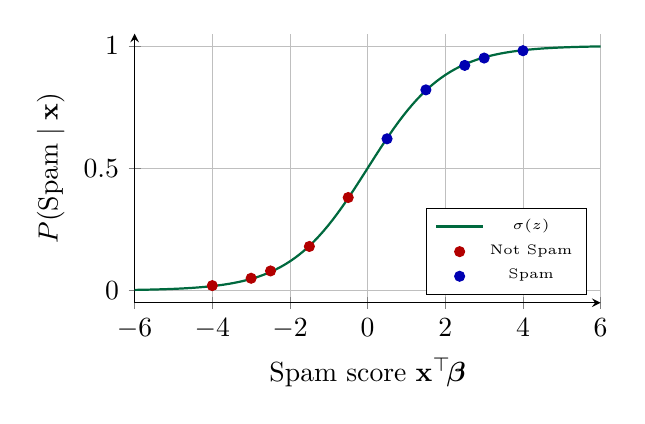
\begin{tikzpicture}
\begin{axis}[
    width=7.5cm, height=5cm,
    xlabel={Spam score $\mathbf{x}^\top\!\bm{\beta}$},
    ylabel={$P(\text{Spam}\mid\mathbf{x})$},
    xmin=-6, xmax=6, ymin=-0.05, ymax=1.05,
    grid=both,
    grid style={line width=.1pt, draw=gray!30},
    major grid style={line width=.2pt, draw=gray!50},
    axis lines=left,
    legend style={font=\tiny, at={(0.97,0.03)}, anchor=south east},
]
\addplot[domain=-6:6, samples=100, color=mantis, thick]
  {1/(1+exp(-x))};
\addplot[only marks, mark=*, mark size=1.8pt, color=red!70!black]
  coordinates {(-4,0.02)(-3,0.05)(-2.5,0.08)(-1.5,0.18)(-0.5,0.38)};
\addplot[only marks, mark=*, mark size=1.8pt, color=blue!70!black]
  coordinates {(0.5,0.62)(1.5,0.82)(2.5,0.92)(3,0.95)(4,0.98)};
\legend{$\sigma(z)$, Not Spam, Spam}
\end{axis}
\end{tikzpicture}
\end{columns}

\end{frame}

% ==================================================================
\section{Why Not Just Use Linear Regression?}
% ==================================================================

% ------------------------------------------------------------------
\begin{frame}{Two Constraints a Probability Must Satisfy}

We need a target function $p(\mathbf{x}) = P(Y=1\mid\mathbf{x})$.

\bigskip

Unlike regression, $p$ is \textbf{not linear}. It must obey:

\bigskip

\begin{block}{1. Boundedness}
$0 \le p(\mathbf{x}) \le 1$ \quad (it is a probability).
\end{block}

\begin{block}{2. Diminishing Sensitivity}
When $p(\mathbf{x}) \approx 1$, a small change in $\mathbf{x}$ should barely
move $p$. \\[4pt]
When $p(\mathbf{x}) \approx 0.5$, the same change has a much larger effect.
\end{block}

\bigskip

We need a \textbf{transformation} that turns a linear function into something satisfying both constraints.

\end{frame}

% ------------------------------------------------------------------
\begin{frame}{The Logit Transformation}

\textbf{Idea:} map $p$ to the \emph{log-odds}, bounded in both directions.

$$\operatorname{logit}(p) = \log\!\left(\frac{p}{1-p}\right)$$

\bigskip

Set this equal to a linear predictor:

$$\log\!\left(\frac{p}{1-p}\right) = \beta_0 + \mathbf{x}^\top\bm{\beta}$$

\bigskip

Hence the name \textbf{logistic regression}.

\end{frame}

% ------------------------------------------------------------------
\begin{frame}{Deriving the Sigmoid Function}

Solve for $p$:

\begin{align*}
\frac{p}{1-p} &= e^{\beta_0 + \mathbf{x}^\top\bm{\beta}} \\[6pt]
p\!\left(1 + e^{\beta_0 + \mathbf{x}^\top\bm{\beta}}\right) &= e^{\beta_0 + \mathbf{x}^\top\bm{\beta}} \\[6pt]
p(\mathbf{x};\beta_0,\bm{\beta})
  &= \frac{1}{1 + e^{-(\beta_0 + \mathbf{x}^\top\bm{\beta})}}
\end{align*}

\bigskip

This is the \textbf{sigmoid (logistic) function}:

$$\boxed{\sigma(z) = \frac{1}{1+e^{-z}}}$$

\end{frame}

% ==================================================================
\section{Decision Boundaries}
% ==================================================================

% ------------------------------------------------------------------
\begin{frame}{From Probabilities to Predictions}

\textbf{Classification rule:} predict $Y=1$ when $p \ge 0.5$, i.e.\
$$\beta_0 + \mathbf{x}^\top\bm{\beta} \ge 0.$$

\bigskip

\textbf{Result:} logistic regression gives a \textbf{linear classifier}.

\bigskip

\begin{block}{Decision Boundary}
The set $\{\mathbf{x} : \beta_0 + \mathbf{x}^\top\bm{\beta} = 0\}$
is a \textbf{hyperplane} in $\R^d$.
\end{block}

Finding the logistic regression parameters $\Leftrightarrow$ finding a linear classifier.

\end{frame}

% ------------------------------------------------------------------
\begin{frame}{Distance from the Decision Boundary}

Let $\mathbf{x}_0$ be any point on the boundary ($\bm{\beta}^\top\mathbf{x}_0 + \beta_0 = 0$).

\bigskip

The \textbf{signed distance} from $\mathbf{x}$ to the boundary:

$$\text{distance}
  = (\mathbf{x}-\mathbf{x}_0)\cdot\frac{\bm{\beta}}{|\bm{\beta}|}
  = \frac{\beta_0 + \mathbf{x}^\top\bm{\beta}}{|\bm{\beta}|}$$

\bigskip

\begin{alertblock}{Interpretation}
Class probabilities depend on the \textbf{distance from the boundary}.
Larger $|\bm{\beta}|$ $\Rightarrow$ probabilities approach 0 or 1 more rapidly.
\end{alertblock}

\end{frame}

% ==================================================================
\section{Choosing a Loss Function}
% ==================================================================

% ------------------------------------------------------------------
\begin{frame}{The 0-1 Loss: Simple but Intractable}

\textbf{Natural idea:} count misclassifications.

$$\hat{\mathcal{R}}_n(\bm{\beta})
  = \frac{1}{n}\sum_{i=1}^{n}
    \mathbf{1}_{Y_i \ne \mathbf{1}_{X_i^\top\bm{\beta}\ge 0}}$$

\bigskip

\textbf{Problem:}
\begin{itemize}
  \item \textbf{Not convex} in $\bm{\beta}$.
  \item \textbf{Not differentiable}.
  \item Minimisation is \textbf{NP-hard} in general.
\end{itemize}

\bigskip

We need a \textbf{convex surrogate}.

\end{frame}

% ------------------------------------------------------------------
\begin{frame}{The Logistic Loss}

Replace the 0-1 loss with a smooth, convex alternative:

$$\ell(\hat{y},\, y)
  = y\log(1+e^{-\hat{y}}) + (1-y)\log(1+e^{\hat{y}})$$

\bigskip

\begin{block}{Logistic Regression Estimator}
$$\hat{\bm{\beta}}_{\text{logit}}
  = \underset{\bm{\beta}\in\R^d}{\arg\min}\;
    \frac{1}{n}\sum_{i=1}^{n}\ell(\mathbf{X}_i^\top\bm{\beta},\, Y_i)$$
\end{block}

\bigskip

\textbf{Key advantage over hinge loss:} the logistic loss has a
\textbf{probabilistic interpretation} via $P(Y=1\mid X)$.

\end{frame}

% ==================================================================
\section{Maximum Likelihood Interpretation}
% ==================================================================

% ------------------------------------------------------------------
\begin{frame}{A Bernoulli Model}

Model the conditional distribution:

\begin{align*}
P(Y=1\mid X=\mathbf{x}) &= \sigma(\bm{\theta}^\top\mathbf{x}) \\[4pt]
P(Y=0\mid X=\mathbf{x}) &= 1 - \sigma(\bm{\theta}^\top\mathbf{x})
\end{align*}

Compact form:

$$P(Y=y\mid X=\mathbf{x})
  = \sigma(\bm{\theta}^\top\mathbf{x})^{y}\,
    [1-\sigma(\bm{\theta}^\top\mathbf{x})]^{1-y}$$

\end{frame}

% ------------------------------------------------------------------
\begin{frame}{Log-Likelihood}

For i.i.d.\ data the \textbf{log-likelihood} is:

$$LL(\bm{\theta})
  = \sum_{i=1}^{n}\bigl[
      y^{(i)}\log\sigma(\bm{\theta}^\top\mathbf{x}^{(i)})
    + (1-y^{(i)})\log(1-\sigma(\bm{\theta}^\top\mathbf{x}^{(i)}))
    \bigr]$$

\end{frame}

% ------------------------------------------------------------------
\begin{frame}{Logistic Loss = Negative Log-Likelihood}

Using the identity $\sigma(-z) = 1 - \sigma(z)$:

\begin{align*}
-\!\log\sigma(z)       &= \log(1+e^{-z}) \\
-\!\log(1-\sigma(z))   &= \log(1+e^{z})
\end{align*}

Therefore:

$$\boxed{-LL(\bm{\theta})
  = \sum_{i=1}^{n}\ell\!\bigl(\hat{y}^{(i)},\, y^{(i)}\bigr)}$$

\bigskip

\begin{alertblock}{Key Equivalence}
Minimising the logistic loss $\;\Longleftrightarrow\;$
Maximising the log-likelihood under a Bernoulli model.
\end{alertblock}

\end{frame}

% ==================================================================
\section{Computing the Gradient}
% ==================================================================

% ------------------------------------------------------------------
\begin{frame}{Derivative of the Sigmoid}

$$\frac{d}{dz}\sigma(z)
  = \frac{e^{-z}}{(1+e^{-z})^2}
  = \sigma(z)\,(1-\sigma(z))$$

\bigskip

Chain rule for the parameters:

$$\frac{\partial}{\partial\theta_j}\sigma(\bm{\theta}^\top\mathbf{x})
  = \sigma(\bm{\theta}^\top\mathbf{x})\,
    (1-\sigma(\bm{\theta}^\top\mathbf{x}))\,x_j$$

\end{frame}

% ------------------------------------------------------------------
\begin{frame}{Gradient of the Log-Likelihood}

For a \textbf{single} data point:

$$\frac{\partial LL}{\partial\theta_j}
  = \bigl[y - \sigma(\bm{\theta}^\top\mathbf{x})\bigr]\,x_j$$

\bigskip

Summing over the dataset:

$$\frac{\partial LL(\bm{\theta})}{\partial\theta_j}
  = \sum_{i=1}^{n}
    \bigl[y^{(i)} - \sigma(\bm{\theta}^\top\mathbf{x}^{(i)})\bigr]\,x_j^{(i)}$$

\bigskip

\textbf{Matrix form:}

$$\boxed{\nabla LL(\bm{\theta})
  = \mathbf{X}^\top\!\bigl(\mathbf{y} - \sigma(\mathbf{X}\bm{\theta})\bigr)}$$

\end{frame}

% ==================================================================
\section{Optimisation}
% ==================================================================

% ------------------------------------------------------------------
\begin{frame}{No Closed-Form Solution}

Setting $\nabla\hat{\mathcal{R}}_n(\bm{\beta})=0$ yields a
\textbf{non-linear} system with no closed-form solution.

\bigskip

\textbf{Good news:} the problem is \textbf{convex}.

$$\frac{\partial^2\ell(\hat y, y)}{\partial\hat y^2}
  = \sigma(\hat y)\,(1-\sigma(\hat y)) > 0$$

\begin{itemize}
  \item Strictly convex $\Rightarrow$ \textbf{unique} minimum.
  \item Solvable by gradient descent/ascent, Newton's method, SGD.
\end{itemize}

\end{frame}

% ------------------------------------------------------------------
\begin{frame}{Gradient Ascent Update Rule}

To \textbf{maximise} the log-likelihood:

$$\bm{\theta} \;\leftarrow\; \bm{\theta} + \alpha\,\nabla LL(\bm{\theta})$$

where $\alpha > 0$ is the learning rate.

\bigskip

\begin{itemize}
  \item $\alpha$ too large $\Rightarrow$ oscillation
  \item $\alpha$ too small $\Rightarrow$ slow convergence
  \item Iterate until $\|\Delta\bm{\theta}\| < \varepsilon$
\end{itemize}

\end{frame}

% ==================================================================
\section{Regularisation}
% ==================================================================

% ------------------------------------------------------------------
\begin{frame}{Preventing Overfitting}

When $d > n$ (more features than samples), logistic regression can
\textbf{overfit}.

\bigskip

\textbf{Fix:} add an L2 penalty.

\begin{block}{L2-Regularised Logistic Regression}
$$\hat{\bm{\beta}}_{\text{ridge}}
  = \underset{\bm{\beta}\in\R^d}{\arg\min}\left\{
    \frac{1}{n}\sum_{i=1}^{n}\ell(\mathbf{X}_i^\top\bm{\beta},Y_i)
    + \lambda\|\bm{\beta}\|_2^2
  \right\}$$
\end{block}

\bigskip

$\lambda > 0$ controls the bias-variance trade-off:
\begin{itemize}
  \item Larger $\lambda$ $\Rightarrow$ more shrinkage, less overfitting.
  \item Smaller $\lambda$ $\Rightarrow$ closer to unregularised fit.
\end{itemize}

\end{frame}

% ==================================================================
\section{Putting It All Together}
% ==================================================================

% ------------------------------------------------------------------
\begin{frame}{The Training Algorithm}

\begin{block}{Logistic Regression via Gradient Ascent}
\begin{enumerate}
  \item \textbf{Input:} $\{(\mathbf{x}^{(i)}, y^{(i)})\}_{i=1}^n$,
        learning rate $\eta$
  \item Initialise $\bm{\theta} \leftarrow \mathbf{0}$
  \item \textbf{Repeat:}
    \begin{enumerate}
      \item[3a.] Compute gradient:
        $\;\nabla LL = \mathbf{X}^\top(\mathbf{y}-\sigma(\mathbf{X}\bm{\theta}))$
      \item[3b.] Update:
        $\;\bm{\theta} \leftarrow \bm{\theta} + \eta\,\nabla LL$
    \end{enumerate}
  \item \textbf{Until} $\|\Delta\bm{\theta}\| < \varepsilon$
  \item \textbf{Output:} $\bm{\theta}$
\end{enumerate}
\end{block}

\end{frame}

% ------------------------------------------------------------------
\begin{frame}{Recap: The Full Story}

\begin{enumerate}
  \item \textbf{Problem:} predict a binary outcome from features.
  \item \textbf{Model:} the logit transform makes probabilities linear
        $\Rightarrow$ sigmoid function.
  \item \textbf{Geometry:} the decision boundary is a hyperplane.
  \item \textbf{Loss:} the 0-1 loss is intractable; the logistic loss
        is convex \emph{and} equals the negative log-likelihood.
  \item \textbf{Gradient:}
        $\nabla LL = \mathbf{X}^\top(\mathbf{y}-\sigma(\mathbf{X}\bm{\theta}))$.
  \item \textbf{Optimisation:} gradient ascent converges to the unique
        solution.
  \item \textbf{Regularisation:} L2 penalty prevents overfitting.
\end{enumerate}

\end{frame}

% ------------------------------------------------------------------
{
\setbeamercolor{background canvas}{bg=mantis}
\setbeamercolor{normal text}{fg=white}
\usebeamercolor[fg]{normal text}
\begin{frame}[c]
\centering
\Huge\textbf{Questions?}
\end{frame}
}

\end{document}
